%%%%%%%%%%%%%%%%%%%%%%%%%%%%%%%%%%%%%%%%%%%%%%%%%%%%%%%%%%%%%%%%%%%%%%%%%%%%%%%%
%2345678901234567890123456789012345678901234567890123456789012345678901234567890
%        1         2         3         4         5         6         7         8

\documentclass[letterpaper, 10 pt, conference]{ieeeconf}  % Comment this line out
                                                          % if you need a4paper
%\documentclass[a4paper, 10pt, conference]{ieeeconf}      % Use this line for a4
                                                          % paper

\IEEEoverridecommandlockouts                              % This command is only
                                                          % needed if you want to
                                                          % use the \thanks command
\overrideIEEEmargins
% See the \addtolength command later in the file to balance the column lengths
% on the last page of the document



% The following packages can be found on http:\\www.ctan.org
%\usepackage{graphics} % for pdf, bitmapped graphics files
%\usepackage{epsfig} % for postscript graphics files
%\usepackage{mathptmx} % assumes new font selection scheme installed
%\usepackage{times} % assumes new font selection scheme installed
%\usepackage{amsmath} % assumes amsmath package installed
%\usepackage{amssymb}  % assumes amsmath package installed

\title{\LARGE \bf
Decentralised market-based strategy for cooperative multi-robot exploration 
}

%\author{ \parbox{3 in}{\centering autor1*
%         \thanks{*Use the $\backslash$thanks command to put information here}\\
%         Faculty of Electrical Engineering, Mathematics and Computer Science\\
%         University of Twente\\
%         7500 AE Enschede, The Netherlands\\
%         {\tt\small h.kwakernaak@autsubmit.com}}
%         \hspace*{ 0.5 in}
%         \parbox{3 in}{ \centering autor2**
%         \thanks{**The footnote marks may be inserted manually}\\
%        Department of Electrical Engineering \\
%         Wright State University\\
%         Dayton, OH 45435, USA\\
%         {\tt\small pmisra@cs.wright.edu}}
%}
\author{Ana Batinovic, Juraj Orsulic, Stjepan Bogdan
	\thanks{Authors are with the University of Zagreb, Faculty of Electrical Engineering  and Computing, LARICS Laboratory for Robotics and Intelligent Control Systems, Unska 3, 10000 Zagreb, Croatia
        {\tt\small (ana.batinovic, juraj.orsulic, stjepan.bogdan) at fer.hr}}}%

\begin{document}



\maketitle
\thispagestyle{empty}
\pagestyle{empty}


%%%%%%%%%%%%%%%%%%%%%%%%%%%%%%%%%%%%%%%%%%%%%%%%%%%%%%%%%%%%%%%%%%%%%%%%%%%%%%%%
\begin{abstract}

This work presents a novel approach to autonomous decentralised multi-robot frontier exploration and mapping of an unknown area based on the market model. The exploration algorithm enables mobile robots to communicate among each other, to negotiate and to become dispersed in the environment. Mobile robot team simultaneously explores the environment, discovers frontier points (points on the border between the explored and unexplored space in map), negotiates by fully connected graph and event-based communication. During the negotiation process mobile robots exchange information just about frontier points, what reduces amount of exchange information. The main goal is to allocate the mobile robots to target frontier points in the environment by minimising overall exploration time. The proposed strategy has been implemented in simulation environment and compared with a centralised market model strategy. The simulation results demonstrate better behaviour for the decentralised multi-robot strategy in the terms of total exploration time and path length. 

\end{abstract}

 
%%%%%%%%%%%%%%%%%%%%%%%%%%%%%%%%%%%%%%%%%%%%%%%%%%%%%%%%%%%%%%%%%%%%%%%%%%%%%%%%
\section{INTRODUCTION}
Analysis and synthesis of decentralised multi-robot systems belong to core robotics problems that draw significant attention in last few decades. The coordination of a mobile robots team during the exploration of an unknown area is a common problem encountered in many applications, such as search and rescue \cite{rescue}, cleaning \cite{cleaning1}, \cite{cleaning2}, warehousing \cite{Wurman}, or planetary exploration \cite{planetary}, to name a few. Due to the fact that autonomous multi-robot systems are entering society domain and as such will interact with people on daily basis, development of reliable coordination algorithms becomes inevitable.

 Like in the human world, robots can be more effective when they work together. Moreover, a robot team can accomplish a predefined task much quicker than a single robot can \cite{free-market}. Another advantage of mobile robot teams arises from possibility to merge overlapping sensor information, which in turn can help to compensate for sensor uncertainty \cite{segmentation}.
If is done properly, multi-robot coordination can lead to i) task accomplishment in the shortest possible time, ii) increased robustness, iii) higher map quality (in case of exploration task), and finally iv) the completion of tasks impossible for a single robot to perform \cite{survey-analysis}.

We consider the problem of an autonomous multi-robot exploration with decentralised coordination strategy based on market model. Mobile robot's laser scan and odometry represent an input data for a Simultaneous Localisation and Mapping module. In this work we focus on graph SLAM method - Google Cartographer \cite{cartographer} which uses the ground truth mobile robot pose (\textit {perfect localisation}) from the Stage simulator \cite{Stage}. Besides a map building and perfect localisation, the module contains a frontier detection described in \cite{juraj}. A result of the frontier detection are the points on the border of the explored and unexplored space in the environment - \textit{frontier points} shown in the Fig. \ref{fig:environment}. The decentralised strategy based on market model module acquires the filtered frontier points and assigns mobile robots to target points. Then the algorithm for path planning navigates mobile robot toward the target point (Fig. \ref{fig:exploration-strategy}).      

\begin{figure}[t]
	\centering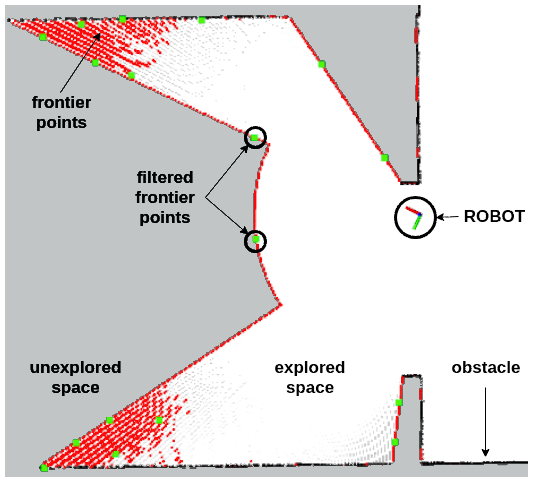
\includegraphics[width=0.85\columnwidth]{frontier_rviz_vol3.png}
	\caption {The description of the environment. A 2D map is represented by occupancy grid that divides the map into cells: the white cells describe explored and grey cells unexplored space, while the black ones define obstacles. The frontier detector publishes frontier points (red) and filter module publishes filtered frontier points (green).}
	\label{fig:environment}
\end{figure}

\begin{figure}[t]
    \centering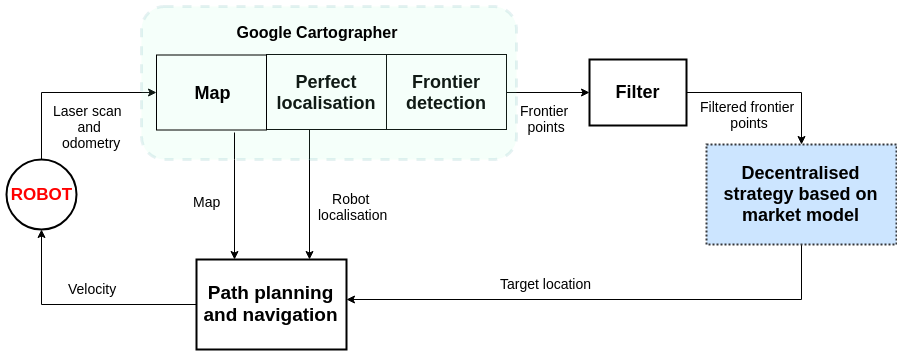
\includegraphics[width=1.0\columnwidth]{diagram_exploration.png}
	\caption{Overall schematic diagram of the exploration algorithm.}
   \label{fig:exploration-strategy}
\end{figure}

Since the main motive is to achieve faster exploration and better coordination among the mobile robots, our decentralised market-based strategy ensures that the mobile robots do not get too close to each other during the exploration. Moreover, the mobile robots are dispersed in the environment to accomplish the mission as fast as possible. It is assumed that communication among the mobile robots is modelled by fully connected graph.

The rest of the paper is organised as follows. The related work is presented in the next section. In Section III the exploration strategy based on market model is going to be explained. Simulation results are in Section IV and in the final section conclusion will be given.

\section{RELATED WORK}

 \subsection{Centralised vs. decentralised}
Assigning robots to target points is achieved either with centralised or decentralised algorithms, for instance, with the nearest frontier approach \cite{Yamauchi}, the cost-utility approach \cite{burgard} or  with an exploration strategy based on a market economy \cite{market-economy}. 

Centralised task assignment for a multi-robot system is often not practical due to communication limits  \cite{free-market}, robustness issues \cite{survey-analysis}, time required for algorithm execution and scalability \cite{Julia}. Generally, in the centralised approach each mobile robot gets tasks assigned from a single central leader using one of the centralised planning algorithm. The communication between the central leader and mobile robots ensures sharing updated information about mobile robot's poses in order to have a real time task allocation. But, an exchange of such a large amount of information can cause the slowness of the process. Previous studies of market-based models indicate that using central system for task assignment suffers from the single point of failure and, furthermore, it relies on complicated protocols \cite{Sheng}. Thus, decentralised bidding models for the multiple mobile robots coordination have been proposed.

Centralised market-based algorithm described in \cite{burgard} improves robustness, but the negotiation process is complex because the coordination of mobile robots is performed by a central executive that creates a global map and executes auction with collected bids from the mobile robots, while in the same time assigning tasks according to the received bids. In other words, a robot (auctioneer) offers a task and other mobile robots compete by giving a bid. One with the highest revenue or the lowest cost is a winner.
The general concept of market-based approaches includes an independence of the mobile robots in terms of planning, and a mobile robots ability to take team resources into account. It is shown in \cite{usporedba} when different team sizes are included, the decentralised market method has an advantage over the centralised approach in terms of distance travelled, and over the behavioural method \cite{behavioural} in terms of computation time.

Hence, the proposed method is based on the market-model that includes an upgrade of the benefit function by adding the occupancy function which makes mobile robots more dispersed in the environment. Moreover, the paper introduces a decentralised market-based strategy that implements event-based communication among mobile robots, reducing amount of information used in negotiation process. 

\subsection{Target point selection}

A popular approach for an unknown area exploration is the frontier based exploration algorithm introduced by Yamauchi \cite{Yamauchi}. The idea is routing mobile robots to the frontier, border that separates explored space form unexplored space in the map. The frontier edges detection can be achieved using RRT (Rapidly Exploring Random Tree) algorithm developed by Hassan Umari and Shayok Mukhopadhyay \cite{Umari}. The RRT algorithm is not only biased towards unexplored regions, but also provides a general approach which can be extended to higher dimensional spaces. However, RRT algorithm proved to be not fast enough in instances when larger parts of the map were discovered, so in this paper, we use frontier detection method that continuously provides frontier \cite{juraj}.   

\section{APPROACH}

The previous work presented a multi-robot exploration system that can efficiently explore unknown terrain, and is robust to robot failures. Our approach attempts to accomplish these performances using strategy based on market model. 
In this paper we determine the target points for each mobile robot in the team using combination of cost, information gain  and frontier occupancy function. 

\subsection{Market-based strategy} 

At the core of our approach is negotiation among mobile robots during the exploration and mapping. The mobile robots exchange information under the assumption of fully connected graph, where all mobile robots communicate with each other and in the negotiation process each mobile robot takes into account the "statements" of the other mobile robots.

Every mobile robot $i$ gets the list of filtered frontier points from the filter module (Fig. \ref{fig:exploration-strategy}):

\begin{equation}
   \boldsymbol{y}=\begin{bmatrix}
    \boldsymbol{y_{0}} & \boldsymbol{y_{1}} & \boldsymbol{y_{2}} & \hdots & \boldsymbol{y_{M}}
\end{bmatrix},
\end{equation}

where $M$ is  the number of filtered frontier points, and every list member is a vector with $x$, $y$ and $z$ components. 

\begin{equation}
   \boldsymbol{y}=\begin{bmatrix}
   \begin{bmatrix}
           x_{0} \\
           y_{0} \\
           z_{0}
   \end{bmatrix}
    \begin{bmatrix}
         x_{1} \\
         y_{1} \\
         z_{1}
    \end{bmatrix}
    \begin{bmatrix}
         x_{2} \\
         y_{2} \\
         z_{2}
    \end{bmatrix}
    \hdots
    \begin{bmatrix}
         x_{M} \\
         y_{M} \\
         z_{M}
    \end{bmatrix}
\end{bmatrix}.
\end{equation}

In this paper we define the weight as a function of the cost, utility and frontier occupancy function. If $i$ is an ordinal number of the mobile robot, and $j$ is an ordinal number of the frontier point then the cost function: $C_{ij}$: $R$ \(\rightarrow \text{$\mathbb{R}^{+}$}\) is a mapping from the set of resources $R$ to a positive real number. $C_{ij}$ describes the cost of $i$th robot to visit $j$th filtered frontier point. The cost can be the function of the time,  energy and so on. In our case the cost is the estimated distance travelled by mobile robot to reach the target frontier point. The estimated distance is approximated using Euclidean distance between the mobile robot position $\boldsymbol{p_{i}}$ and the filtered frontier point position $\boldsymbol{q_{j}}$:

\begin{equation}\small
    C_{ij}=d(\boldsymbol{p_{i}}, \boldsymbol{q_{j}}) = \sqrt{(p_{ix}-q_{jx})^{2}+(p_{iy}-q_{jy})^{2}+(p_{iz}-q_{jz})^{2}}.
    \label{cost}
\end{equation}

The utility function $U_{ij}$:  \(\text{$\mathcal {M}$}\) \(\rightarrow \text{$\mathbb{R}^{+}$}\) returns a positive real number from the occupancy grid \(\text{$\mathcal {M}$}\). The cells of \(\text{$\mathcal {M}$}\) may be marked as explored space, unexplored space or obstacle. The utility function is proportional to the number of the unexplored cells within a fixed distance from the filtered frontier point $j$ in the previous defined radius $r$: 

\begin{equation}
    U_{ij} = \lambda_{u}c,
\end{equation}

where $\lambda_{u}$ is a constant experimentally determined. It is assumed that the mobile robot will detect all unexplored cells around the assigned frontier point after reaching it. 

The frontier occupancy function $F_{ij}$ is 2-dimensional Gaussian function with the position of the peak in the frontier point and with the standard deviations $3\sigma_{x}=r_{f}$ and $3\sigma_{y}=r_{f}$. Moreover, the frontier occupancy function has a value if the frontier point $j$, for which mobile robot $i$ is calculating the weight, is in the range of radius $r_{f}$ from the position of the mobile robot assigned point ($q_{a}$). 

\begin{equation}
    F_{ij} =  \lambda_{f} e^{-\Big[\frac{(q_{jx} - q_{ax})^2}{2\sigma_{x}^2} + \frac{(q_{jy} - q_{ay})^2}{2\sigma_{y}^2}\Big]},
\end{equation}
where $\lambda_{f}$  is also  a constant experimentally determined. The example of the filtered frontier point $j$ and its radii $r$ and $r_{f}$ is shown in Fig. \ref{fig:radijusi}.

\begin{figure}[b!]
	\centering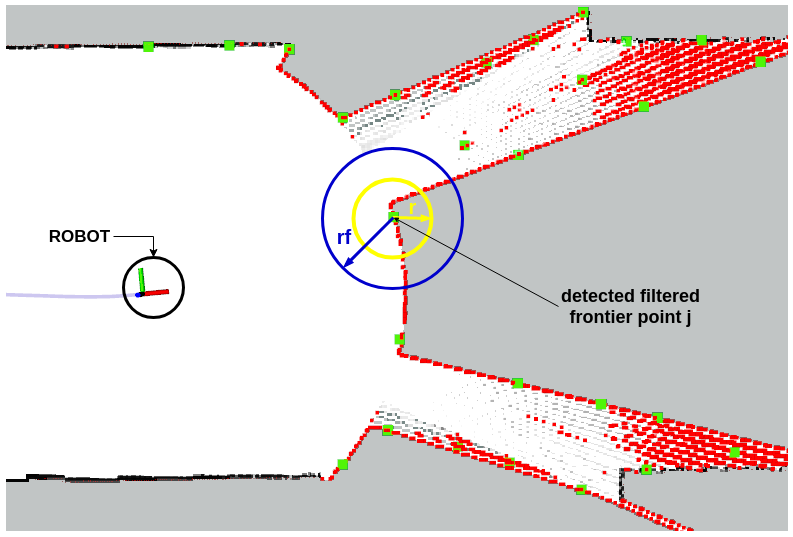
\includegraphics[width=0.85\columnwidth]{rviz_radius_vol3.png}
	\caption{Detected filtered frontier point $j$ and its radii $r$ and $r_{f}$.}
	\label{fig:radijusi}
\end{figure}

For each filtered frontier point $j$ weight $W_{ij}$ of $i$-th mobile robot is calculated as: 
\begin{equation}
   {W}_{ij}= {C_{ij}} - {U_{ij}} + {F_{ij}}.
   \label{weight}
\end{equation}

The weight matrix $\boldsymbol{W}$ ($N\times M$) is formed for $N$ mobile robots and $M$ filtered frontier points: 

\begin{equation}
    \boldsymbol{W} = \begin{bmatrix}
    W_{00} & W_{01} & \hdots & W_{0j} & \hdots & W_{0M}\\
    W_{10} & \ddots & & & & \vdots\\
    \vdots & & \ddots & & &  \vdots \\
    W_{i0} & & & \ddots & & \vdots \\
    \vdots & & & & \ddots & \vdots\\
    W_{N0} & \hdots  & \hdots  & \hdots  & \hdots &    W_{NM}
    \end{bmatrix}.
\end{equation}

Mobile robots exchange the information about the weight for the particular filtered frontier point and make decisions for the future actions. Accordingly the amount of exchanging data is reduced and results in easier and faster communication.
The weight matrix $\boldsymbol{W}$ represents the input into the Hungarian algorithm that finds an optimal assignment solution in polynomial time. The Hungarian algorithm is described in \cite{hungarian} and tested in \cite{comparison}. 

Let the matrix $X$ be the matrix of zeros and ones, where $X[i,j]=1$ iff the mobile robot $i$ is assigned to the frontier point $j$.
Than the optimal task assignment has weight:

\begin{equation}
     {\mathrm{min}}\ \sum_{i} \sum_{j} W_{ij}\ X_{ij},
\end{equation}

anticipating that minimisation of sum could ensure the dispersion of the mobile robots in the environment. 

\begin{algorithm}[H]
\caption{Decentralised strategy for a mobile robot $i$ exploration}
\label{algorithm1}
\begin{algorithmic}[1]
\For{ each filtered frontier point $j$}
\State\hspace{\algorithmicindent} $W_{ij}$ = $C_{ij}$ - $U_{ij}$ + $F_{ij}$
\State\hspace{\algorithmicindent} Send $W_{ij}$ to the other mobile robots.
\State \hspace{\algorithmicindent} Receive the weights from the others.
\State \hspace{\algorithmicindent} Calculate weight matrix $\boldsymbol{W}$.
\State \hspace{\algorithmicindent} Hungarian algorithm ($\boldsymbol{W}$).
\State{\textbf{return} Mobile robot $i$ is assigned to frontier point.}
\EndFor
\end{algorithmic}
\end{algorithm}

Our decentralized strategy is in progress during the robot's motion and there are seven steps for each robot to be executed (Algorithm \ref{algorithm1}).    

When mobile robot $i$ is assigned to frontier point according to line 7 in Algorithm \ref{algorithm1}, the mobile robot starts to follow the planned path and navigate to the target frontier point. Moreover, at the moment when the mobile robot $i$ reaches the target point, a weight calculation request is sent to the other mobile robots, whose responses fill the  weight matrix $\boldsymbol{W}$ (an input to Hungarian algorithm). The described process is executing until the whole environment is explored.

\section{SIMULATION RESULT}

The proposed strategy is implemented and tested using the Robot Operating System (ROS) framework. In order to prove the efficiency of our decentralised strategy, we compared it with coordinated centralised market model described in \cite{burgard}. Experiments were performed in the two different indoor environments (Fig. \ref{fig:scenarios}) with the two, three and five mobile robots. The start pose of the mobile robot was the same for each run. The results are presented as average of 10 runs for each set.

\begin{figure}[t]
	\centering
	\begin{minipage}{\dimexpr.48\columnwidth}
		\centering
		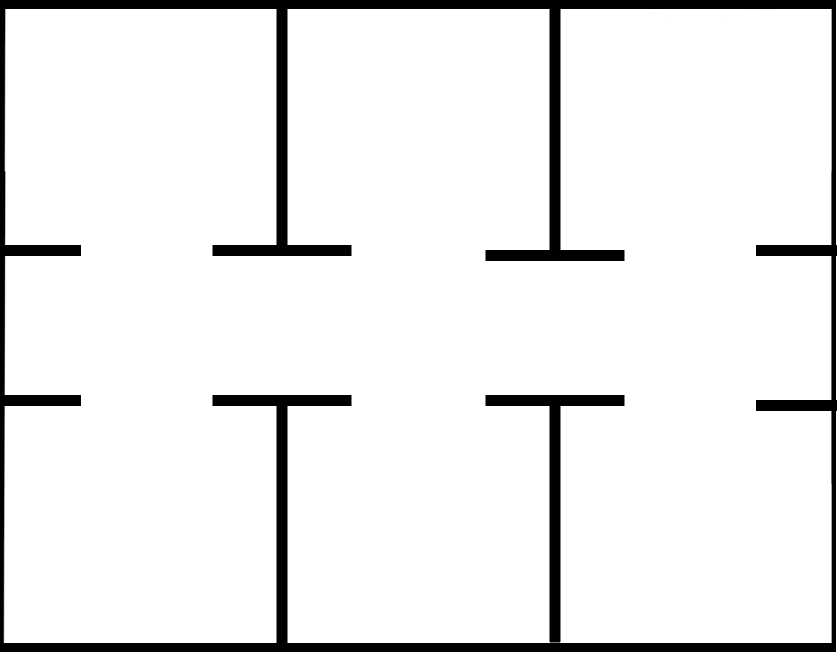
\includegraphics[width=\columnwidth]{office1.png}
		\captionsetup{labelformat=empty}
		\caption*{\boldsymbol{a)}}
		\label{fig:office}
	\end{minipage}%
	\hspace{0.1cm}%
	\begin{minipage}{\dimexpr.48\columnwidth}
		\centering
		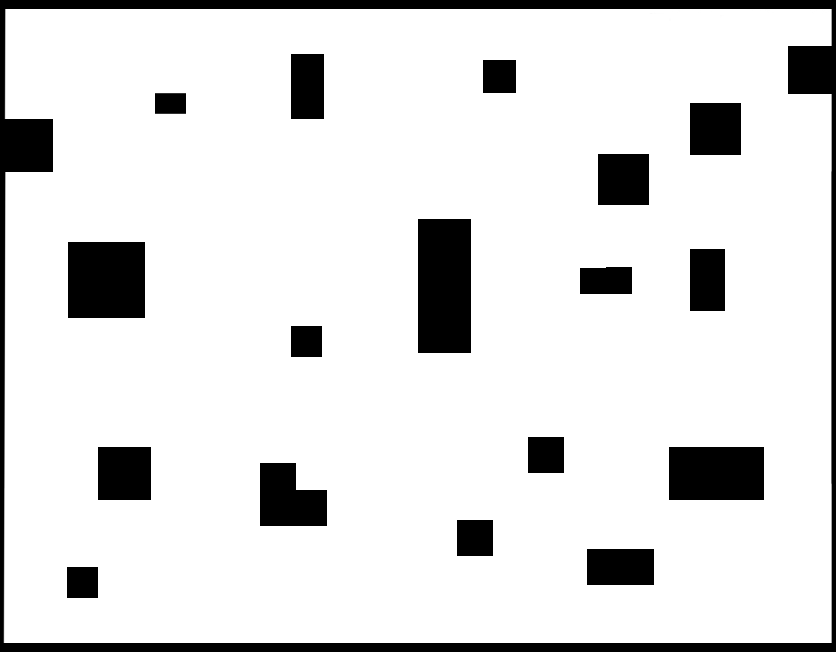
\includegraphics[width=\columnwidth]{unstructured.png}
		\captionsetup{labelformat=empty}
		\caption*{\boldsymbol{b)}}
		\label{fig:unstructured}
	\end{minipage}
 \caption{Benchmark scenarios. The terrains cover the flat surface 40 x 20 $m^{2}$ with static obstacles. \boldsymbol{a)} Office-like scenario; \boldsymbol{b)} Unstructured scenario. }
 \label{fig:scenarios}
\end{figure}
The comparison of the centralised strategy and our decentralised strategy is shown using the indicators defined as follows:

\textbf{Coverage Ratio (CR)}: percentage of the accessible terrain covered by the team. Calculated as:  \( \frac{\text{explored cells} \cdot 100}{\text{accessible cells}} \).

\textbf{Path Length (PL)}: sum of the distance travelled by each robot measured in meters.

\textbf{Total exploration Time (TT)}: time elapsed from the beginning until the end of exploration measured in seconds.\\

First of all, it is interesting to see how the coverage evolves over time. Fig. \ref{fig:office_cent}, Fig. \ref{fig:office_decent}, Fig. \ref{fig:unstruc_cent} and Fig. \ref{fig:unstruc_decent} show \textbf{CR} over time for both centralised and decentralised multi-robot exploration strategies in the office scenario as well as in the unstructured scenario. We report the time it takes to cover 50, 75, 90 and 99 percent of the environment. Obviously, it takes almost the same time to explore a few last cells and 25 percent (from 75 to 90 percent) of the environment. In the both scenarios, decentralised strategy need less time to explore the same percentage of the environment.  

\begin{figure}[b!]
	\centering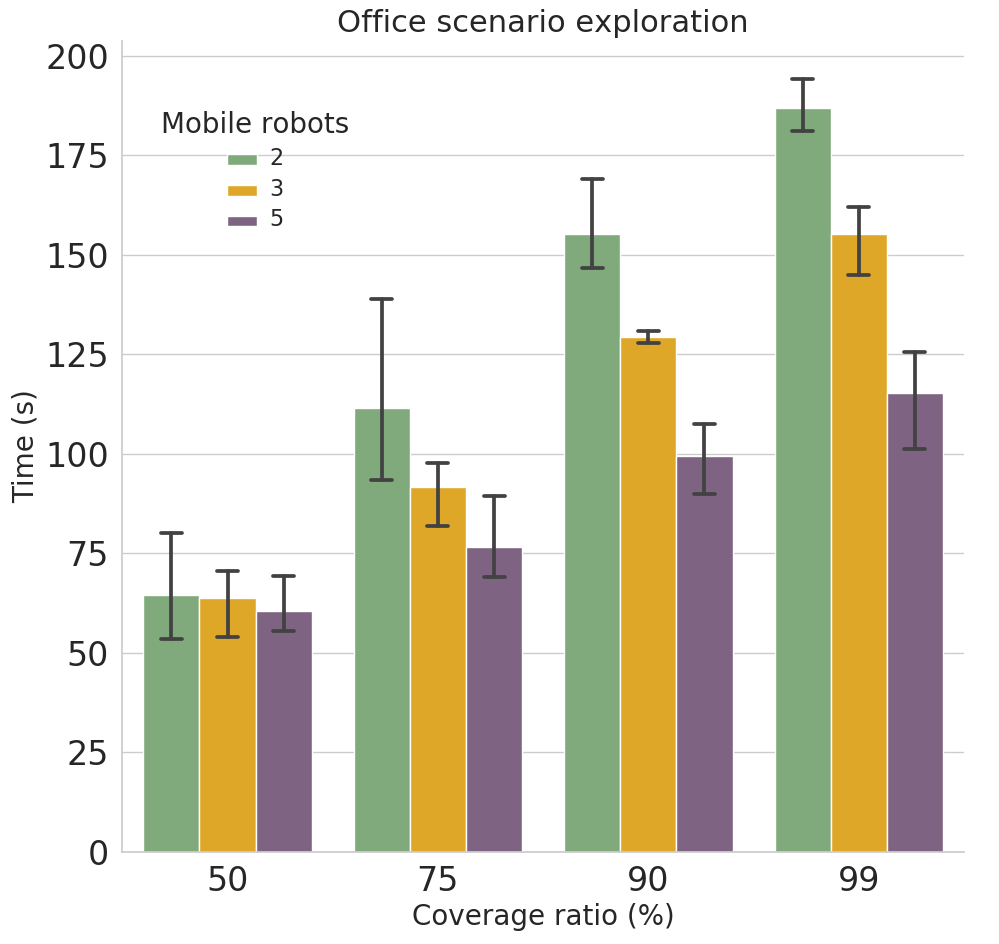
\includegraphics[width=0.9\columnwidth]{office_coverage_cent.png}
	\caption{Coverage ratio over time in the office scenario centralised multi-robot exploration.}
	\label{fig:office_cent}
\end{figure}

\begin{figure}[h!]
	\centering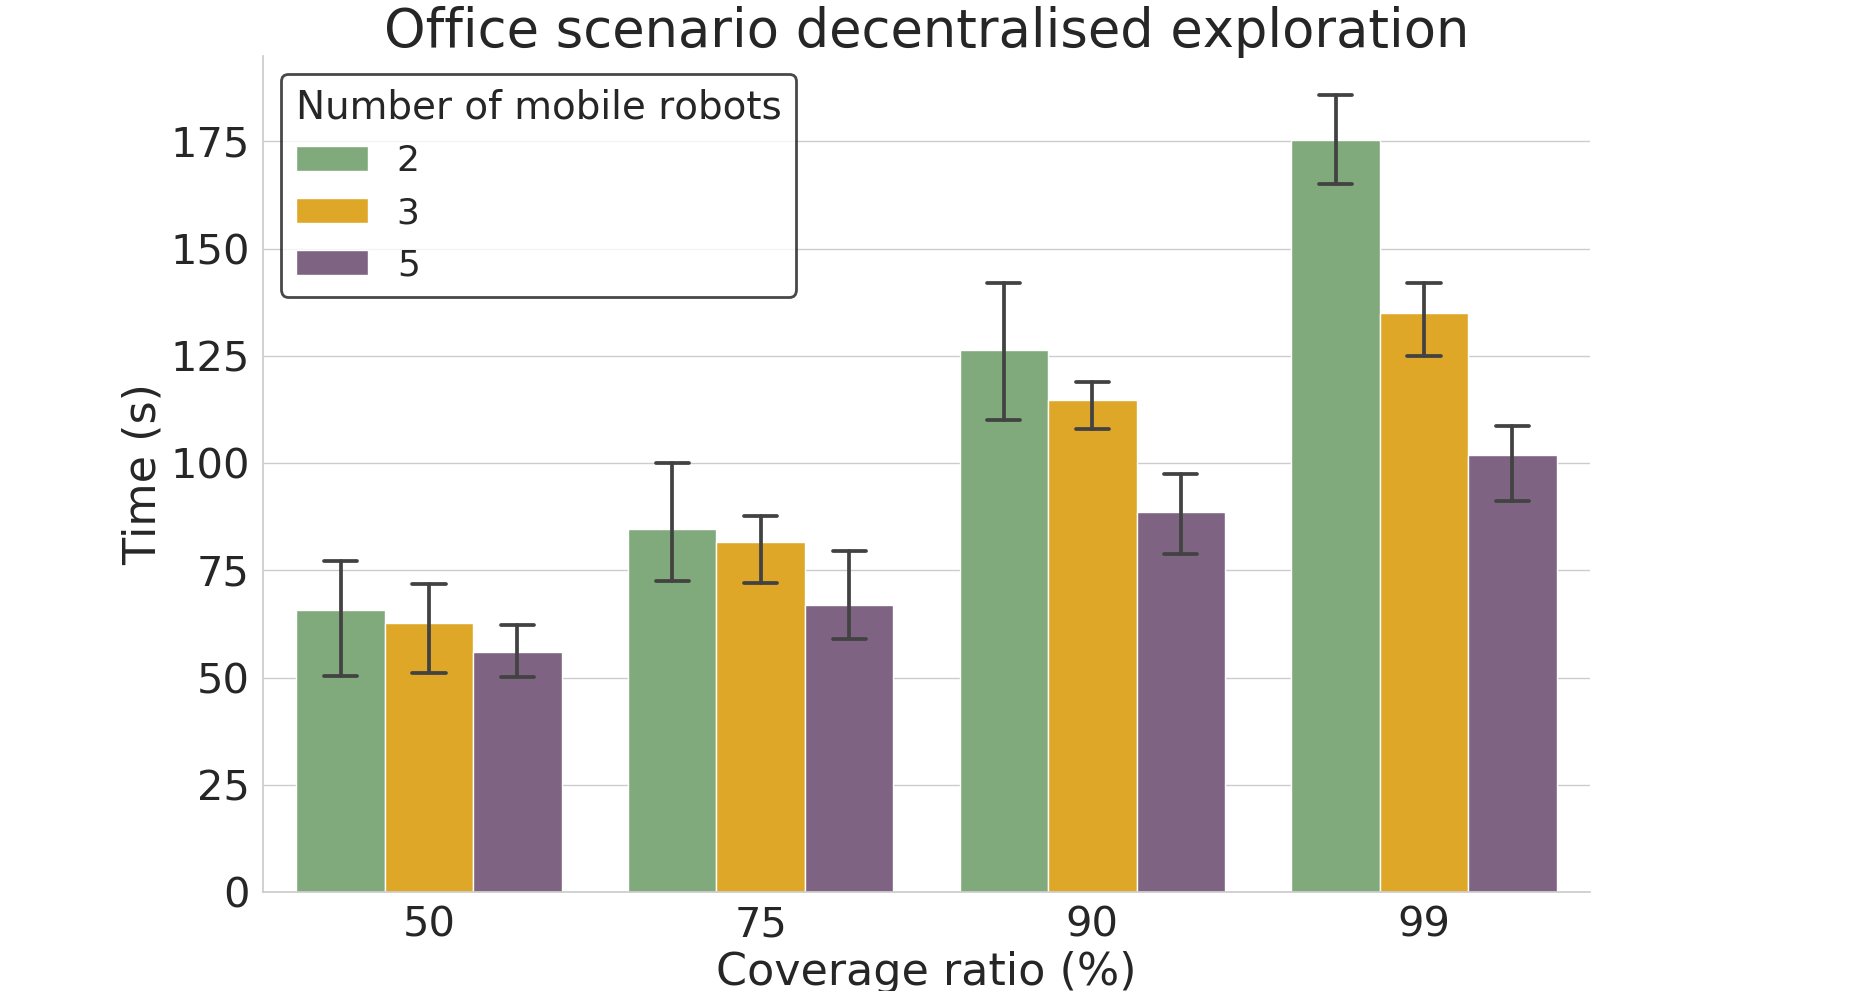
\includegraphics[width=0.9\columnwidth]{office_coverage_decent.png}
	\caption{Coverage ratio over time in the office scenario decentralised multi-robot exploration.}
	\label{fig:office_decent}
\end{figure}

\begin{figure}[h!]
	\centering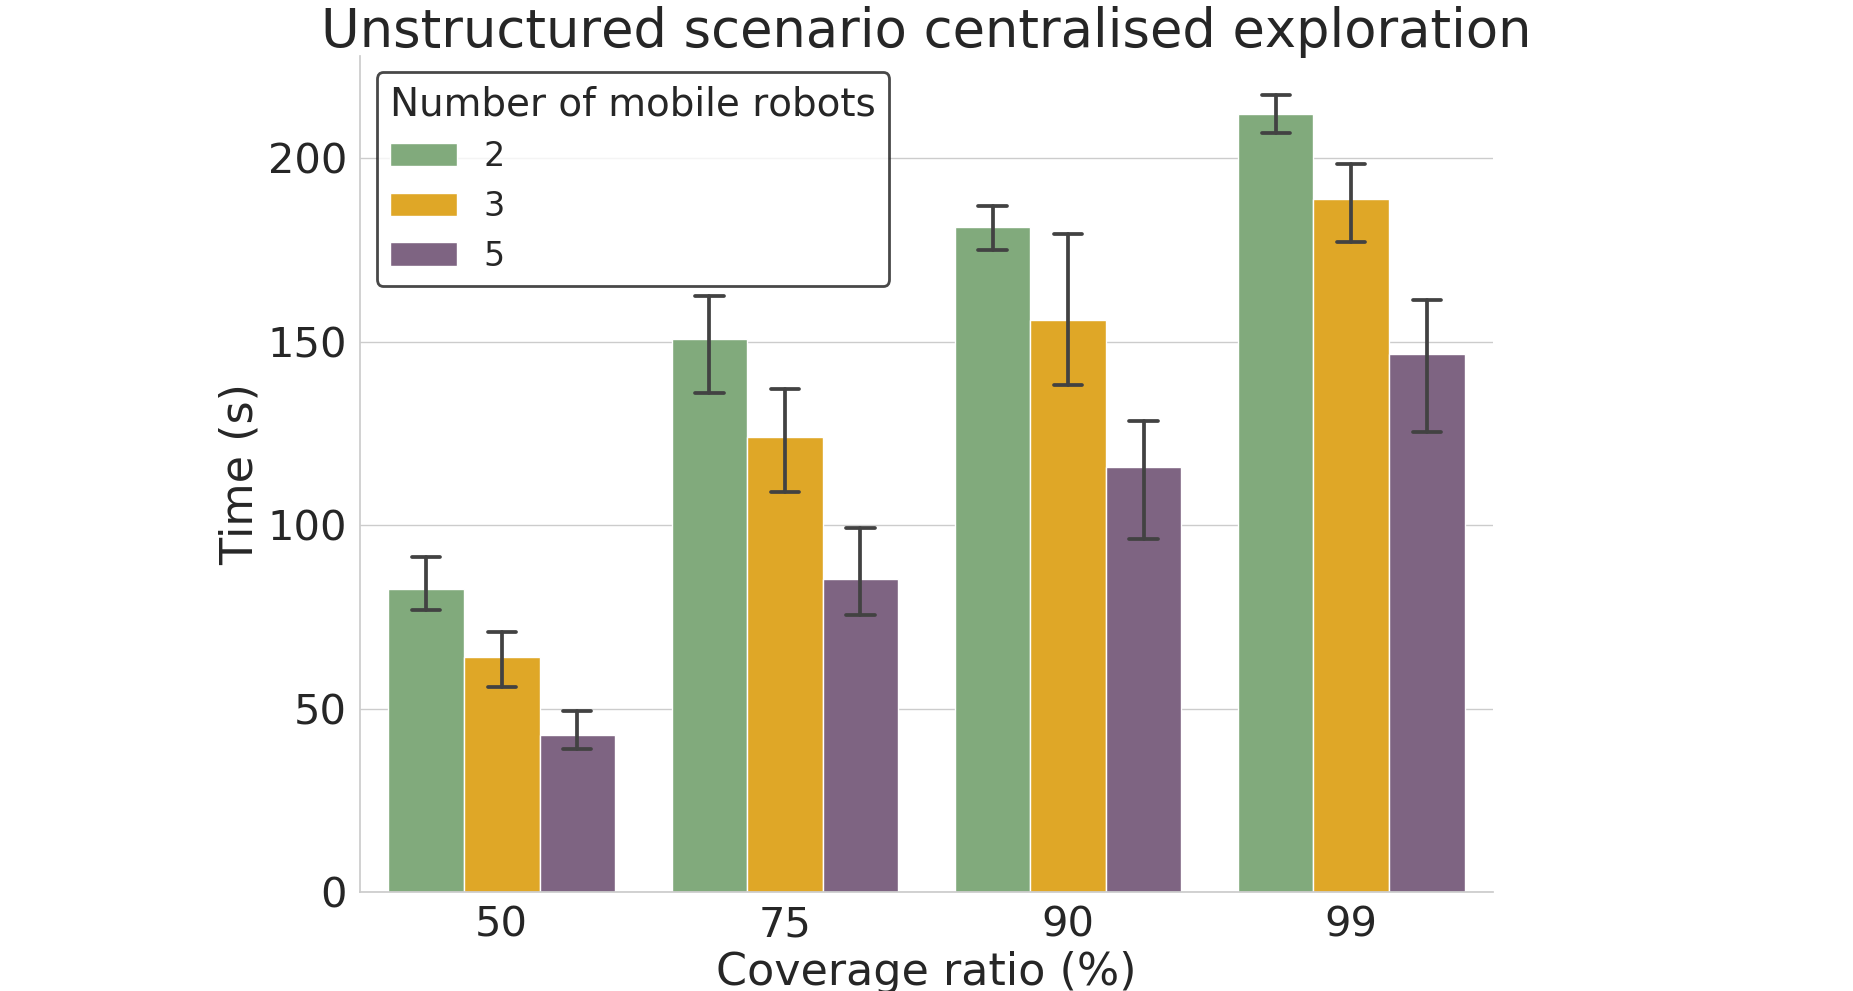
\includegraphics[width=0.9\columnwidth]{unstructured_coverage_cent.png}
	\caption{Coverage ratio over time in the unstructured scenario centralised multi-robot exploration.}
	\label{fig:unstruc_cent}
\end{figure}

\begin{figure}[h!]
	\centering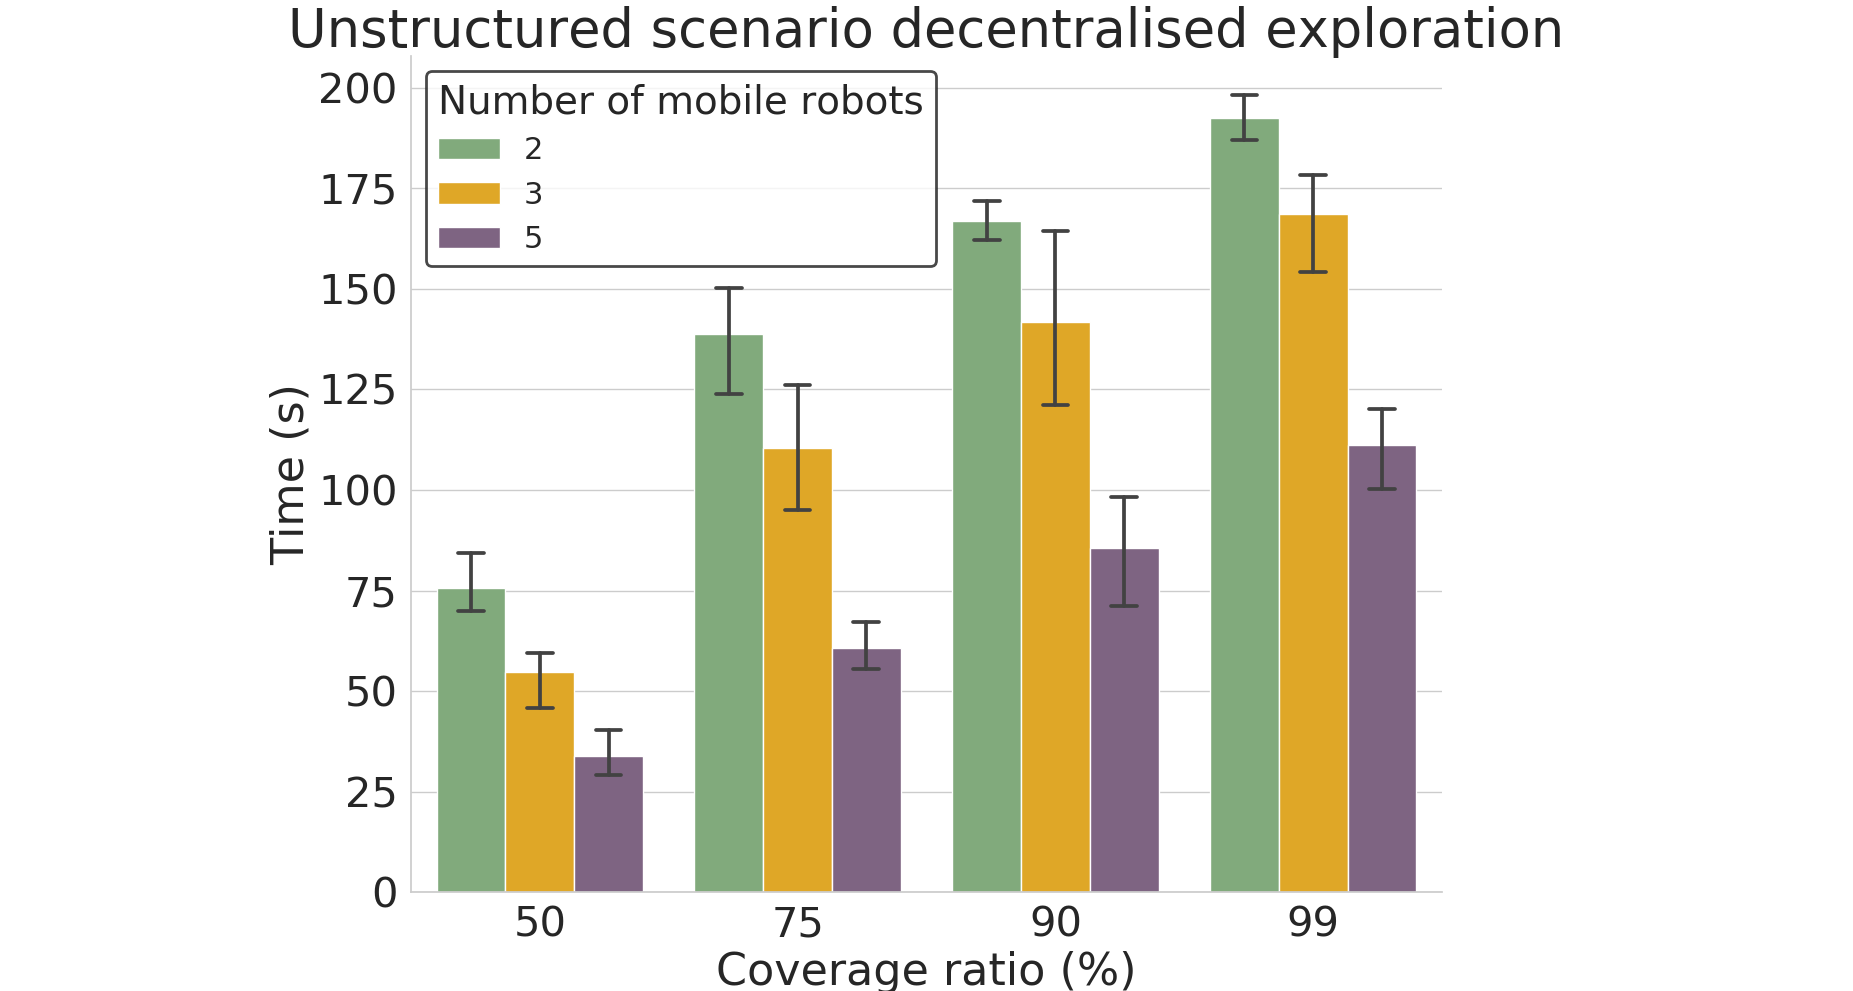
\includegraphics[width=0.9\columnwidth]{unstructured_coverage_decent.png}
	\caption{Coverage ratio over time in the unstructured scenario decentralised multi-robot exploration.}
	\label{fig:unstruc_decent}
\end{figure}

The next parameter of the interest is \textbf{PL} shown in the Fig. \ref{fig:office_path} and Fig. \ref{fig:unstruc_path}. It is shown that the proposed decentralised strategy based on market model gives better results than the centralised strategy from \cite{burgard}, especially in the office scenario for two and three mobile robots. 


When we compare the \textbf{TT} for the both strategies (Fig. \ref{fig:office_tt} and Fig. \ref{fig:unstruc_tt}), it shows that five mobile robots perform better than two and three, while there is a small difference in having three robots instead of two. And still our decentralised strategy performs faster than the centralised. 
\begin{figure}[t]
	\centering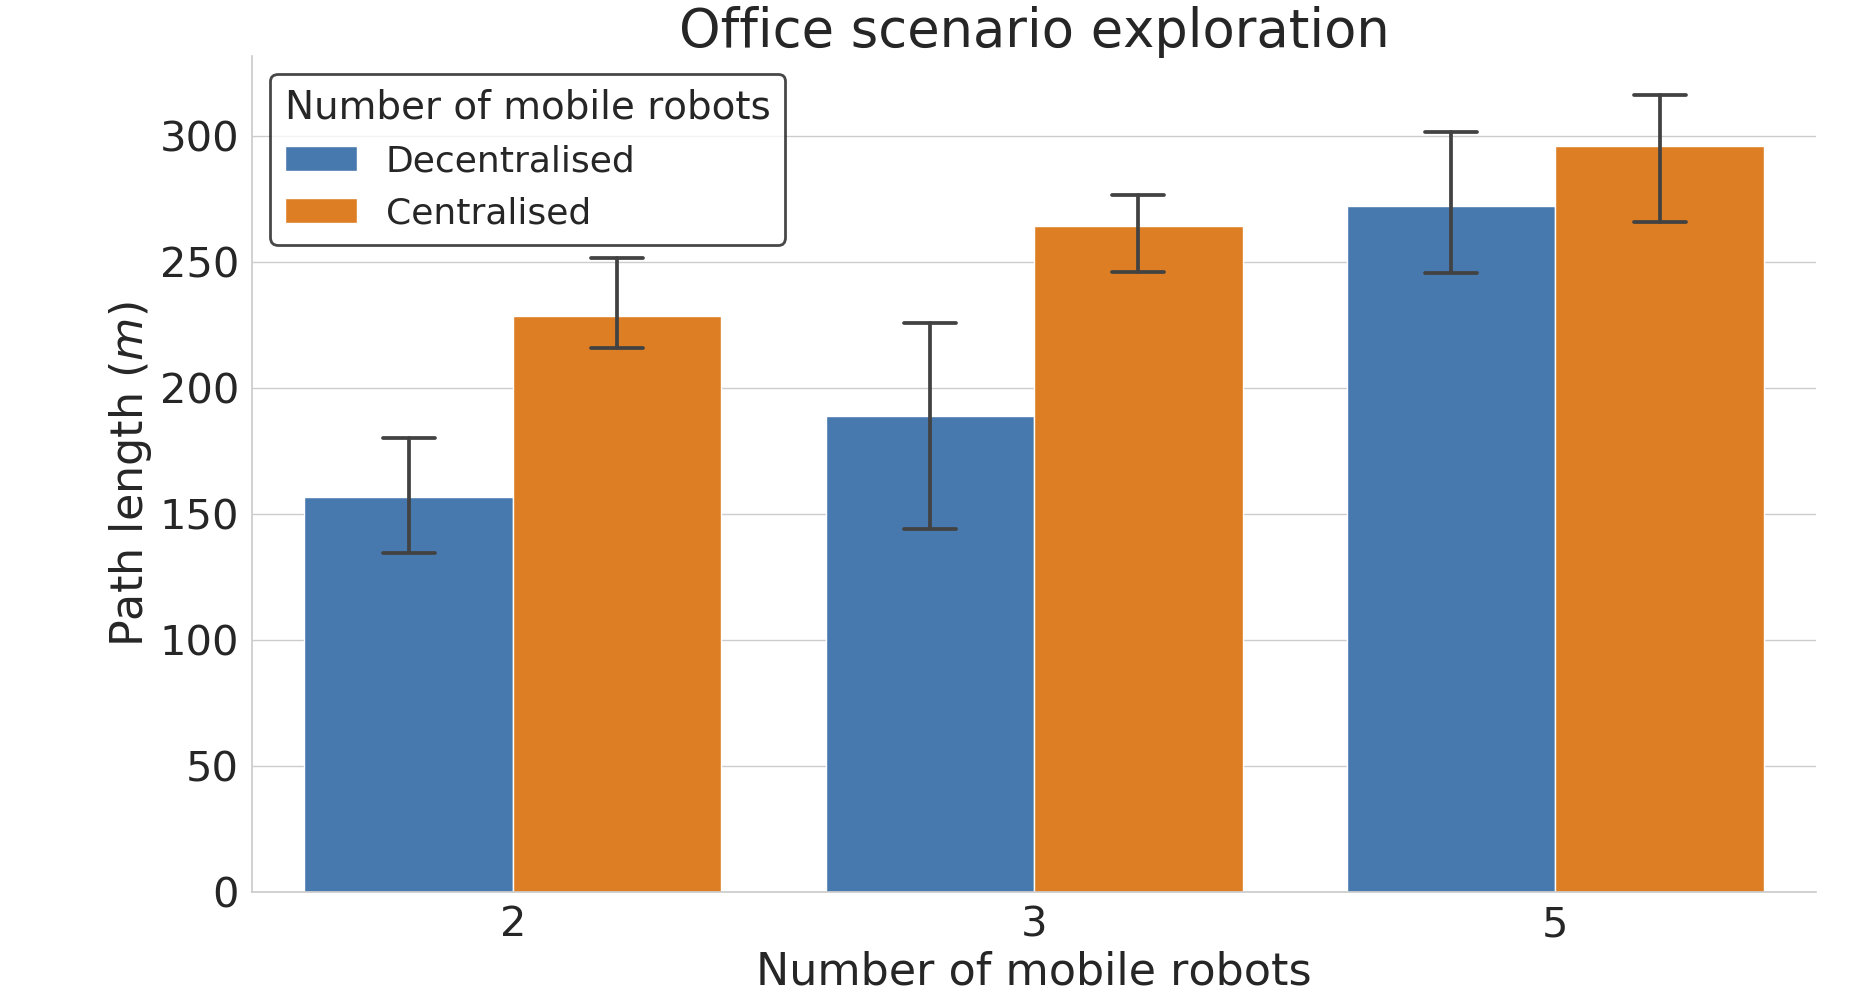
\includegraphics[width=0.9\columnwidth]{office_path.png}
	\caption{Path length in the office scenario for the different size of the robot team.}
	\label{fig:office_path}
\end{figure}

\begin{figure}[t]
	\centering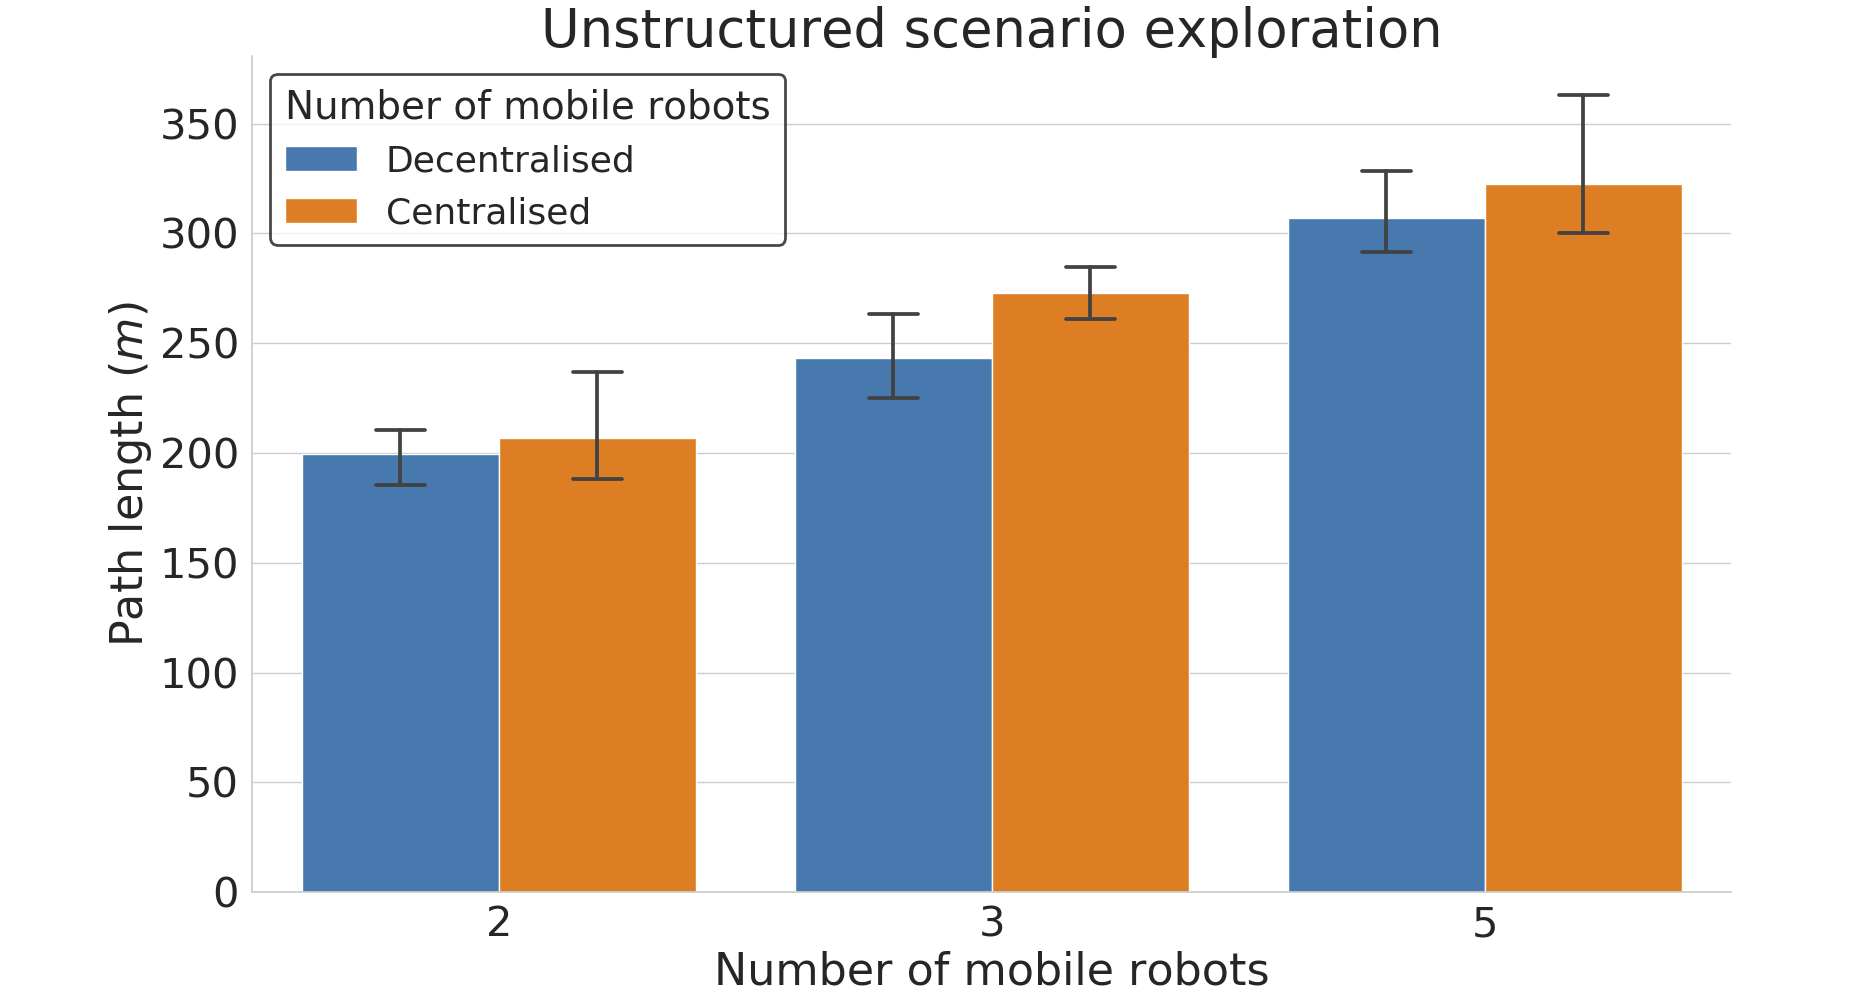
\includegraphics[width=0.9\columnwidth]{unstructured_path.png}
	\caption{Path length in the unstructured scenario for the different size of the robot team.}
	\label{fig:unstruc_path}
\end{figure}

\begin{figure}[t]
	\centering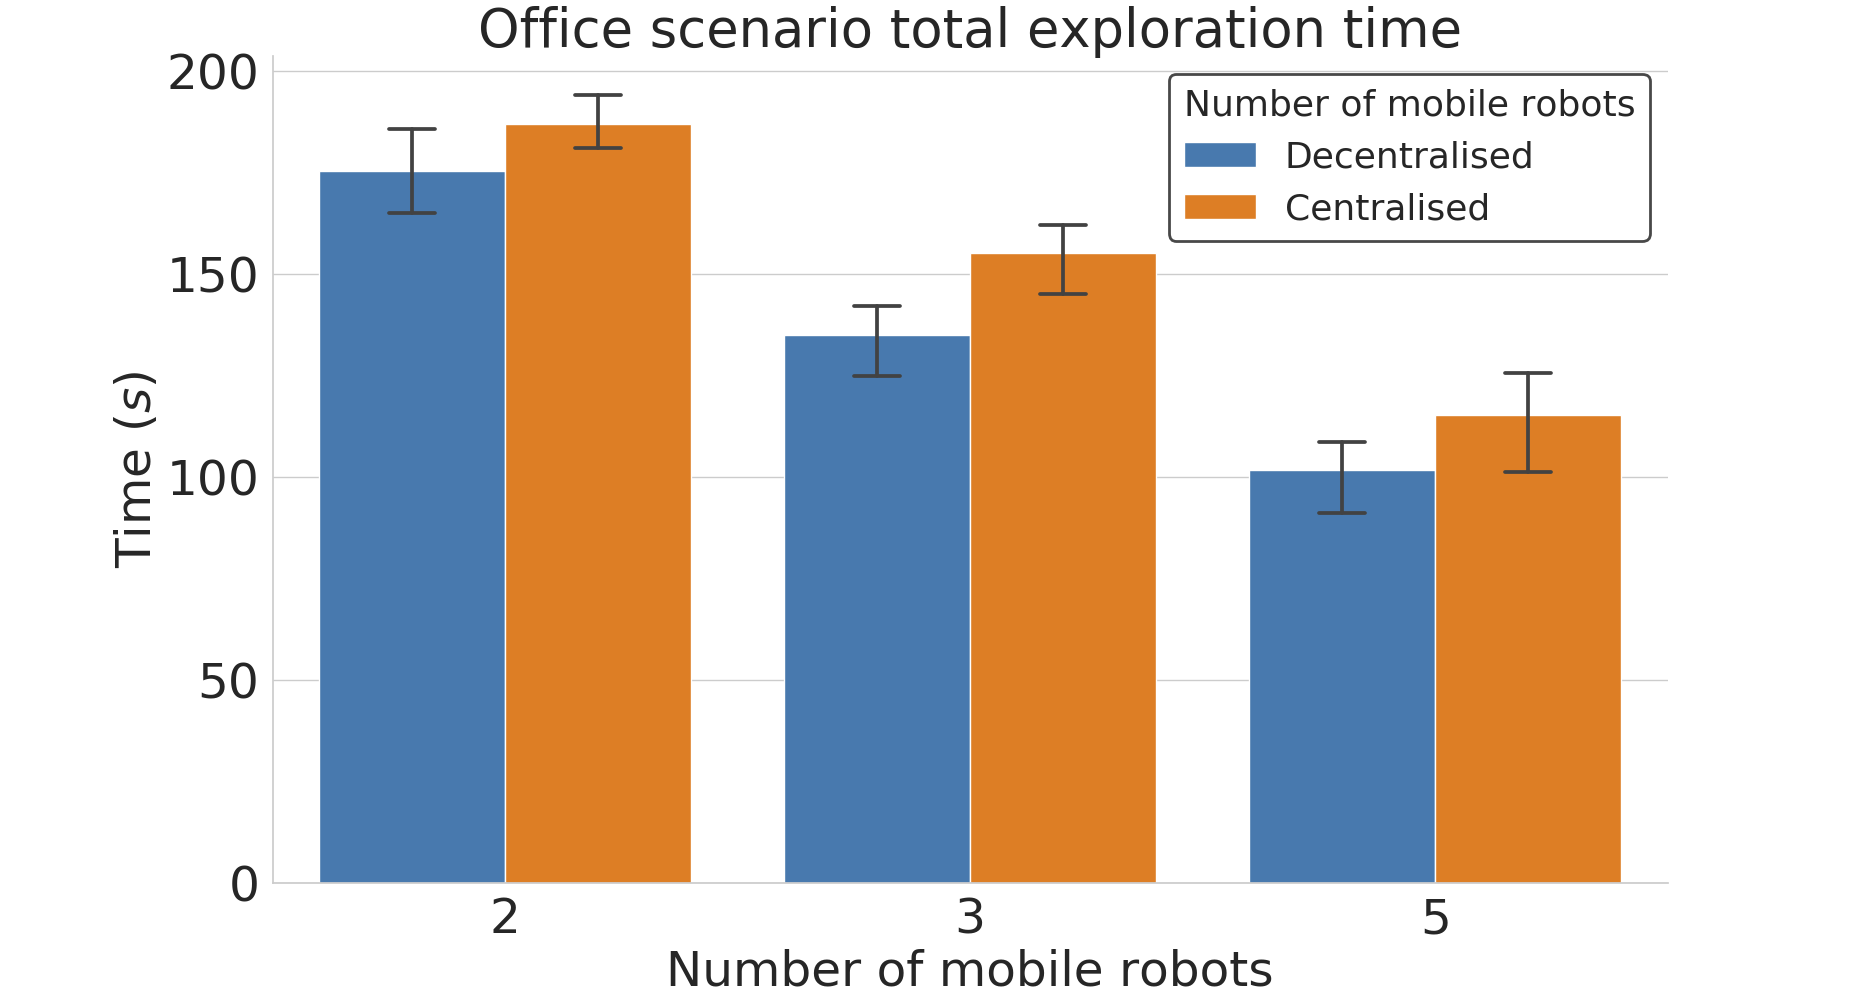
\includegraphics[width=0.9\columnwidth]{office_tt.png}
	\caption{Total time exploration in the office scenario.}
	\label{fig:office_tt}
\end{figure}

\begin{figure}[t]
	\centering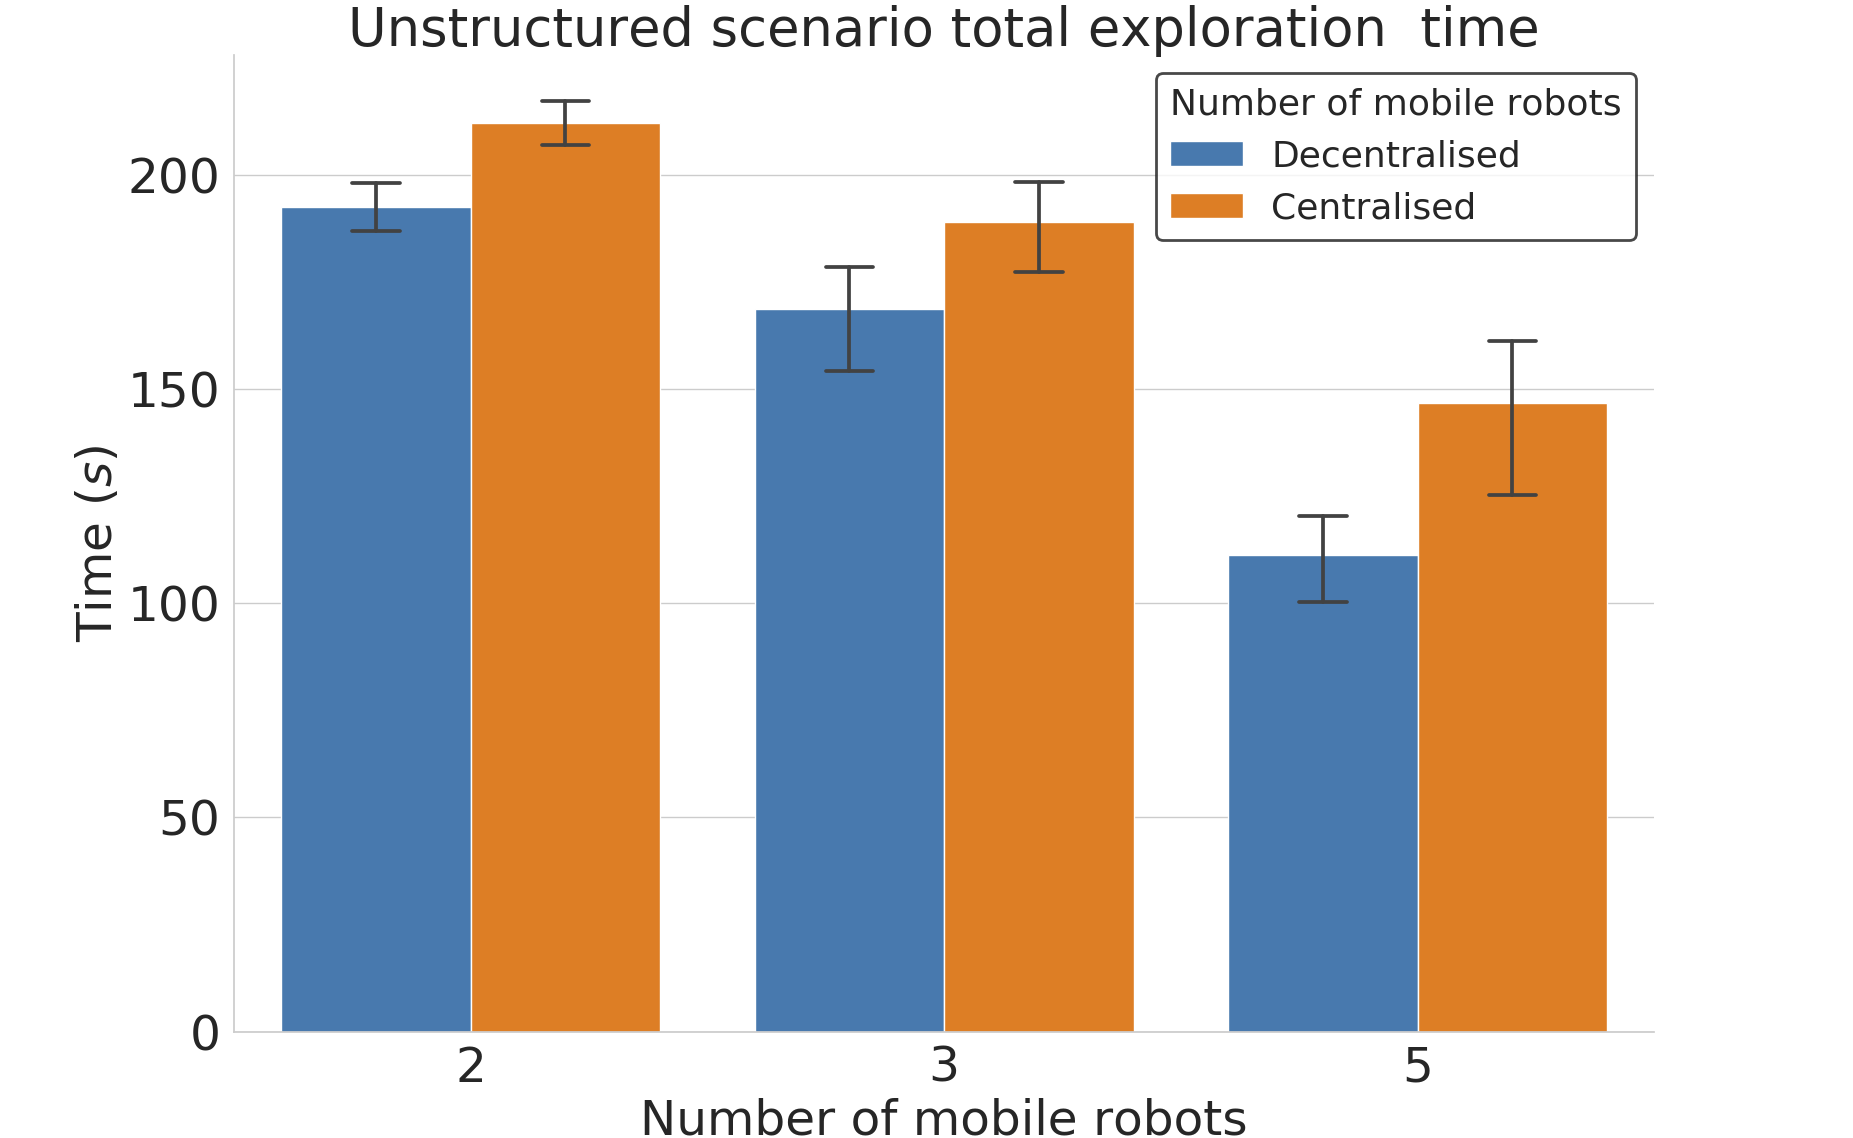
\includegraphics[width=0.9\columnwidth]{unstructured_tt.png}
	\caption{Total time exploration in the unstructured scenario.}
	\label{fig:unstruc_tt}
\end{figure}


\section{CONCLUSION AND FUTURE WORK}

We have presented an approach to autonomous decentralised multi-robot
exploration and mapping based on the market model. This strategy has demonstrated better behaviour compared to the centralised strategy that explicitly coordinates the robots, based on estimates of expected information gain and the cost of exploration. This includes both reduced total exploration time and path length.

However, the approach described in this paper is limited in three aspects. Firstly, we currently assume that the mobile robots begin an exploration from the same start pose. More sophisticated techniques include different randomly generated start poses for each simulation run. Secondly, in this work the filter module reduce the number of the frontier points by removing the points that are too close to each other. We are investigating more sophisticated and efficient filtering, which we believe will improve overall performance significantly. And thirdly, all mobile robots communicate to each other and create a fully connected graph. If we limit the communication range and assume that just the mobile robots close to each other can communicate and negotiate, the exploration can be more effective. 

\addtolength{\textheight}{-12cm}   % This command serves to balance the column lengths
                                  % on the last page of the document manually. It shortens
                                  % the textheight of the last page by a suitable amount.
                                  % This command does not take effect until the next page
                                  % so it should come on the page before the last. Make
                                  % sure that you do not shorten the textheight too much.

%%%%%%%%%%%%%%%%%%%%%%%%%%%%%%%%%%%%%%%%%%%%%%%%%%%%%%%%%%%%%%%%%%%%%%%%%%%%%%%%


\begin{thebibliography}{99}

\bibitem{free-market} B. Dias, S. Stentz, A Free Market Architecture for Distributed Control of a Multirobot System, in 6th International Conference on Intelligent Autonomous Systems, pp. 115-122, 2000.

\bibitem{burgard} W. Burgard, M. Moors, C. Stachniss, and F. Schneider. Coordinated multi-robot exploration. IEEE Transactions on Robotics, 21(3):376–378, 2005.

\bibitem{hungarian} H.W. Kuhn, The hungarian method for the assignment problem, Naval Research Logistics Quarterly, 2(1):83–97, 1955.

\bibitem{planetary} M.J. Matarić and G. Sukhatme, Task-allocation and coordination of
multiple robots for planetary exploration, in Proc. of the Int. Conf. on Advanced Robotics (ICAR), pages 61–70, Budapest, Hungary, 2001.

\bibitem{Yamauchi} B. Yamauchi, Frontier-based exploration using multiple robots, in
Proc. of the Second International Conference on Autonomous Agents, pages 47–53, Minneapolis, MN, USA, 1998.

\bibitem{market-economy} R. Zlot, A.T. Stenz, M.B. Dias, and S. Thayer, Multi-robot exploration controlled by a market economy, in Proc. of the IEEE Int. Conf. on Robotics and Automation (ICRA), Washington, DC, USA, 2002.

\bibitem{rescue} R. Murphy, Human-robot interaction in rescue robotics, IEEE Syst., Man, Cybern., C, Appl. Rev., vol. 34, no. 2, pp. 138–153, May 2004.

\bibitem{cleaning1} H. Endres, W. Feiten, and G. Lawitzky, Field test of a navigation system: autonomous cleaning in supermarkets, in Proc. IEEE Int. Conf. Robot. Autom. (ICRA), pp. 1779–1781, 1998.

\bibitem{cleaning2} P. Pinheiro, E. Cardozo, J. Wainer, and E. RohmerCleaning, Task Planning for an Autonomous Robot in Indoor Places with Multiples Rooms, International Journal of Machine Learning and Computing, Vol. 5, No. 2, April 2015.

\bibitem{segmentation} K. M. Wurm, C. Stachniss, and W. Burgard, Coordinated multi-robot exploration using a segmentation of the environment, in Proc. IEEE/RSJ  International Conference on Intelligent Robots and Systems (IROS), September 2008.

\bibitem{Julia} M. Julia, A. Gil, and O. Reinoso, A comparison of path planning strategies for autonomous exploration and mapping of unknown environments, Autonomous Robots, vol. 33, no. 4, pp. 427–444, 2012. 

\bibitem{comparison} M. Kulich, T. Juchelka, and L. Preucil, Comparison of exploration strategies for multi-robot search, Acta Polytech, 55(3):162, June 2015. 

\bibitem{survey-analysis} M. B. Dias, R. Zlot, N. Kalra,and A. Stentz, Market-based multirobot coordination: A survey and analysis, Proceedings of the IEEE 94 (7), 1257-1270, 2006.

\bibitem{Umari} H.Umari, and S. Mukhopadhyay, Autonomous Robotic Exploration Based on Multiple Rapidly-exploring Randomized Trees,  in Proc. IEEE/RSJ International Conference on Intelligent Robots and Systems (IROS), Vancouver, BC, Canada, September 2017.
  
\bibitem{Sheng} W. Sheng, Q. Yang, S. Ci, and N. Xi, Distributed Multi-robot Coordination Algorithm for Area Exploration and Mapping, IEEE International Conference on Robotics and Automation (ICRA) Workshop on The State-of-the-Art of Mobile Robot Area Coverage, 2004.

\bibitem{usporedba} M. B. Dias, and A. Stentz, A Comparative Study between Centralized, Market-Based, and Behavioral Multirobot Coordination Approaches, in Proceedings of the 2003 IEEE/RSJ  International Conference on In Intelligent Robots and Systems (IROS), Las Vegas, Nevada, October 2003.

\bibitem{Wurman} P. R. Wurman, R. D'Andrea, and M. Mountz, Coordinating hundreds of cooperative, autonomous vehicles in warehouses, in Proc. IAAI'07 Proceedings of the 19th national conference on Innovative applications of artificial intelligence, vol. 2, pp. 1752-1759, Vancouver, British Columbia, Canada, July 2007
 
\bibitem{behavioural} H. Lau, Behavioural approach for multi-robot exploration, Proceedings of. 2003 Australasian Conference on Robotics and Automation, Brisbane, Australia, December 2003

\bibitem{cartographer} W.  Hess,  D.  Kohler,  H.  Rapp,  and  D.  Andor, Real-time  loop  closure in  2d  lidar  slam, inRobotics  and  Automation  (ICRA), 2016  IEEEInternational Conference on. IEEE, 2016, pp. 1271–1278

\bibitem{juraj} J. Orsulic, D. Mikic and Z. Kovacic, Efficient Dense Frontier Detection for 2D GraphSLAM Based on Occupancy Grid Submaps

\bibitem{Stage} W. Woodall, http://wiki.ros.org/stage

\end{thebibliography}

\end{document}
